
\chapter{Markov Chain Monte Carlo}
\label{MCMC}
The main signal extraction presented in \mbox{Chapter \ref{SigEx}}
minimizes the difference between the Monte Carlo and the data, varying
proportions of the various signals and backgrounds and distortions in
the MC (the systematics).  This involves a large number of parameters
and each step is very computationally expensive, making a typical
minimizer such as Minuit \cite{Minuit} impractical.  Instead, we turn
to the Markov Chain Monte Carlo (MCMC) method.  Here we describe the
basic ideas of the method, the particular MCMC algorithm we have
chosen, and why this method is preferable for this problem.

\section{Definitions}
The Markov Chain Monte Carlo (MCMC) method derives from the principles
of Bayesian statistics.  We will not go in to the fundamentals of
this, which can be found in a number of references
\cite{ref:DataAnalysisBook, BayesianIntro}.  But we will need a few
definitions of terms that are commonly used in this field, as the
following discussion will rely on this notation.  In addition, we
define several terms as shorthand or for convenience in the following
discussion.  To illustrate the meaning of these quantities, we look at
a hypothetical problem: we have a model of the weather in Boston, and
wish to test its validity.

\begin{itemize}
\item[ ] $p(x)$ is the probability distribution function (pdf) for x.
  This requires context - if x is Temperature, then $p(x)$ for Boston
  will be different from $p(x)$ for Orlando, which will be very
  different than $p(x)$ for a quark-gluon plasma.
\item[ ] $p(x|y)$ is a conditional probability of x, given y
  (i.e. assuming y is true).  Continuing our example,
  $p(x|\mathrm{summer})$ will have much more weight near 80$^\circ$F
  than $p(x|\mathrm{winter})$.
\item[ ] $\{\vec{x}\}$ is a set of data points.  Individual points
  will be denoted $\vec{x}_i$.  Our example could be a set of
  measurements of temperature and wind speed at various times.
\item[ ] $\{\vec{y}\}$ is a set of simulated events from a Monte Carlo
  based on our model.  Individual points will be denoted $\vec{y}_i$.
\item[ ] $\vec{\alpha}$ is a set of model parameters.  Again,
  individual points will be denoted $\alpha_i$.  Our example could be
  the season and the time of day, so that we are asking our model to
  only look at summer afternoons.
%\item[] A tilde over a variable indicates a ``proposed'' value given
%  by a step in a process, but not necessarily kept.  For example,
%  $\tilde{\alpha}_j$ is the proposed value for the j$^{\mathrm{th}}$
%  parameter
\end{itemize}


\section{Markov Chain Monte Carlo}
The method of the Markov Chain Monte Carlo is a combination of two
parts: a ``Markov Chain'', a random walk with the next step only
dependent on the current step; and a ``Monte Carlo'', a simulation
method using repeated random sampling.  It requires a known relation
between the data distribution and a set of model parameters, giving
$p(\vec{x}|\vec{\alpha})$ and a measured set of data points
$\{\vec{x}\}$; it returns information about the values of
$\vec{\alpha}$, i.e. about the probability distribution
$p(\vec{\alpha}|\{\vec{x}\})$ (called the posterior distribution).
The method randomly walks through the space of $\vec{\alpha}$ in a
particular way (which defines the algorithm but is always a Markov
Chain) and returns a random sample (the Monte Carlo aspect) from
$p(\vec{\alpha}|\{\vec{x}\})$, usually called a ``chain''.

This random sample is akin to the output of a ``normal'' fitter, most
of which assume that this distribution is Gaussian to report some
value $\alpha_i \pm \sigma_{\alpha_i}$ for each model parameter.  To
convert from $p(\vec{\alpha}|\{\vec{x}\})$ to $\alpha_i \pm
\sigma_{\alpha_i}$, we need merely assume that
$p(\vec{\alpha}|\{\vec{x}\})$ is Gaussian near its maximum and, for
each parameter individually, either fit with a Gaussian or numerically
compute the mean and standard deviation of the random sample.  But
with the MCMC methods, we have the flexibility of looking directly at
the probability distribution if we wish.  

The method relies on having a way to define the probability that a
data set was drawn from a distribution, since we will be varying our
distribution as we vary $\vec{\alpha}$.  This is most naturally done
with the Likelihood function, described in the next section.  In the
context of the overall analysis, the question arises of how to
describe $p(\vec{x}|\vec{\alpha})$ at all, given the complexity of the
experiment forces us to rely on Monte Carlo simulations.  We will
delay answering this question until \mbox{Chapter \ref{SigEx}}; for
the rest of the chapter we will assume we have this available to us.

There are many MCMC algorithms (see \cite{ref:DataAnalysisBook,
NealReport} for an overview), differing mainly in how the random walk
through parameter space is implemented.  The simplest, and first to be
discussed, is the Metropolis algorithm \cite{MetropolisPaper}.  This
is the one we will use.  Many factors went in to this decision. The
most proiminent are that the more advanced algorithms often require
the analytic derivative of $p(\vec{x}|\vec{\alpha})$, which we do not
have available, or they require more evaluations of
$p(\vec{x}|\vec{\alpha})$, which we will find is very computationally
expensive to evaluate.  In addition, the Metropolis algorithm was used
is the previous SNO analysis presented in \cite{NCDPRL}, so the SNO
collaboration had experience with the algorithm and had already
approved its use.

\section{Extended Log Likelihood}
\label{ExtendedLogLikelihood}
In general terms, we have an experiment that produces a set of data
points $\{\vec{x}_i\}$, with each point consisting of a number of
values.  Assuming that these data points represent
statistically independent events (interactions in our detector), we
can say that these are random draws from some probability distrubtion
$p(\vec{x}|\vec{\alpha})$, where $\vec{\alpha}$ is a set of parameters
describing this distrubtion's shape.  Since it is a probability
distribution, we have $\int_{\mathrm{all}\ \vec{x}}
p(\vec{x}|\vec{\alpha}) = 1$ for any $\vec{\alpha}$.  We don't know
this distrubtion a priori (else we wouldn't need to do the
experiment), but we assume that we have a good enough understanding of
the system that our ignorance can be characterized by the set of
parameters $\vec{\alpha}$.  Our goal is now to find the $\vec{\alpha}$
that best matches our data.

As per usual, the Likelihood is defined as the product of the
probabilites of drawing each of the points.
\begin{equation}
\label{SimpleLikelihood}
\mathcal{L}(\vec{\alpha}) = \prod_i^n\ p(\vec{x}_i|\vec{\alpha})
\end{equation}
This gives a measure of the ``probability'' that the data set was
drawn from $p(\vec{x}|\vec{\alpha})$, in the sense that the better that
$p(\vec{x}|\vec{\alpha})$ agrees with the data, the larger $\mathcal{L}$.

Unfortunately, this is too simple.  First, this assumes that we are
drawing from a normalized probability density function (PDF), when in
reality the number of events in our data set is very important.
Second, many of the elements of $\vec{\alpha}$ are constrained by
external measurements.  The former is dealt with by using the Extended
Likelihood, which penalizes differences between the number of events
expected and the number of data events, and the latter by adding terms
to the likelihood.

The Extended Likelihood is a standard prescription.  We now have a
``PDF'' $N \cdot p(\vec{x}|\vec{\alpha})$, which will have $N$ events
in it - integrating across the distribution gives $N\cdot1$.  To
incorporate this, we multipy the Likelihood in \mbox{equation
\ref{SimpleLikelihood}} by a Poisson distribution for the number of
data events, with mean equal to the number of events $N$ in the
``PDF'' (which is now no longer normalized to one).  We call the
number of data events $n$ and we will drop the quotes around PDF from
now on, with the knowledge that we are now talking about $N
p(\vec{x}|\vec{\alpha})$ instead of $p(\vec{x}|\vec{\alpha})$.  This
gives
\begin{equation}
\mathrm{EL}(\vec{\alpha}) = \frac{N^n e^{-N}}{n!} \mathcal{L}(\vec{\alpha})
= \frac{N^n e^{-N}}{n!} \prod_i^n\ p(\vec{x}_i|\vec{\alpha})
\end{equation}
We will later take the logarithm of this for computational reasons.
Quickly evaluating that logarithm gives
\begin{equation}
\log(\mathrm{EL}) = n \log(N) - N - \log(n!) + \sum_i^n \log(p(\vec{x}_i
| \vec{\alpha})) = \sum_i^n \log(N p(\vec{x}_i | \vec{\alpha})) - N -
\log(n!)
\end{equation}
Note that $n$ is a constant (since the set of data points is fixed),
while $N$ is not (since this is a parameter of our PDF, which we will
later take to be part of $\vec{\alpha}$).

The constraint terms are external measurements for our parameters,
giving independent information about the values the parameter can
take.  We simply multiply our $\mathcal{L}$ by the (normalized) pdf
that corresponds to the measurement.  This is stating that we have a
prior distribution for that parameter, so that our external
information tells us what we think the probability distribution for
that parameter should be. In our analysis, these take one of three
forms: a Gaussian, a ``two sided Gaussian'', and a covariance matrix.

The simplest and most common case is the Gaussian.  If a parameter
$\alpha_j$ has a value $\bar{\alpha}_j \pm \sigma$, then we multiply
$\mathcal{L}$ by a gaussian distribution
\begin{equation}
p(\alpha_j) =
\frac{1}{\sqrt{2\pi}\sigma}\exp\left(-\frac{(\alpha_j-\bar{\alpha}_j)^2}
{2\sigma^2}\right)
\end{equation}

The ``two-sided Gaussian'' is the case of asymmetric uncertainties,
i.e. a measured value of $\bar{\alpha}^{+\sigma_+}_{-\sigma_-}$.  This
corresponds to a Gaussian with one value of $\sigma$ above the mean
and a different one below, so we multiply $\mathcal{L}$ by
\begin{equation}
p(\alpha_j) = \frac{\sqrt{2}}{\sqrt{\pi}(\sigma_+ + \sigma_-)}\left\{
\begin{array}{rl}
\exp\left(-\frac{(\alpha_j-\bar{\alpha}_j)^2}
{2\sigma_-^2}\right) & \text{if } \alpha_j \leq \bar{\alpha}_j\\
\exp\left(-\frac{(\alpha_j-\bar{\alpha}_j)^2}
{2\sigma_+^2}\right) & \text{if } \alpha_j > \bar{\alpha}_j
\end{array} \right.
\end{equation}

A covariance matrix is somewhat more complicated, as it links the
values of several parameters.  It corresponds to a multi-dimensional
Gaussian.  Given an $m \times m$ covariance matrix $\mathbf{\Sigma}$
linking $m$ parameters (label them $\vec{\beta}$)
\begin{equation}
p(\vec{\beta}) = \frac{1}{(2 \pi)^{m/2} |\mathbf{\Sigma}|^{1/2}}
  \exp\left(-\frac{1}{2} (\vec{\beta}-\bar{\vec{\beta}})^T
  \mathbf{\Sigma}^{-1} (\vec{\beta}-\bar{\vec{\beta}})\right)
\end{equation}

For ease of computation, and computational accuracy on a
finite-precision machine, we take the logarithm of the product of the
extended likelihood and the constraints.  Since $\log(x)$ is a
monotonically increasing function of $x$, maximizing one is equivalent
to maximizing the other.  We drop all terms that are constants and
hence do not contribute to the maximization process to end up with the
Extended Log Likelihood:
\begin{equation}
\mathrm{ELL}(\vec{\alpha}) = \log(\mathrm{EL}) + \sum_{constraints}
\log(p(\vec{\alpha})) = \sum_{i=0}^{n} \log(N p(\vec{x}_i | \vec{y}))
- N + \sum_{constraints} \log(p(\vec{\alpha}))
\end{equation}
When the constraint terms are expanded, in general the normalization
coefficients, being constant, are dropped.

In sum, we now have a way of measuring the probability that our data
set $\{\vec{x}\}$ was drawn from the distribution characterized by
$\vec{\alpha}$, taking in to account the known constraints on
$\vec{\alpha}$.  How this $\mathrm{ELL}$ changes as we change
$\vec{\alpha}$ will tell us how we want to direct our random walk
through parameter space, as codified in the Metropolis algorithm.

\section{Metropolis Algorithm}
The Metropolis algorithm consists of a loop which walks across the
parameter space of $\vec{\alpha}$.  At the end of the $i^{th}$ step,
it will have the parameter values $\vec{\alpha}_i$.  The $(i+1)^{th}$
step starts by varying each of the parameters by adding a random draw
from a Gaussian with $\mu=0$ and $\sigma=\sigma_{\alpha_j}$, i.e. each
parameter is varied around its current position with a width specific
to that parameter (determined before the process starts, see
\mbox{Section \ref{rott:StepSizeFinding}}).  This creates a
``proposed'' step $\vec{\alpha}_{i+1}^{prop}$.  The Extended
Likelihood (including all constraints, so
$\exp(\mathrm{EL}(\vec{\alpha})$) is then compared between the
previous and the current step by taking the ratio $\displaystyle
p(\mathrm{step}) =
\frac{EL(\vec{\alpha}_{i+1}^{prop})}{EL(\vec{\alpha}_i)}$.  A random
number is drawn from the uniform distribution between $0$ and $1$,
call it $\mathrm{rand}(0,1)$.  If $\mathrm{rand}(0,1) <
p(\mathrm{step})$ then we keep the proposed value and set
$\vec{\alpha}_{i+1} = \vec{\alpha}_{i+1}^{prop}$, if not we don't take
the step and keep our old one, so $\vec{\alpha}_{i+1} =
\vec{\alpha}_i$.  This latter point is important - the repetition in
our data set of ``better points'' is a large part of what gives rise
to the useful behavior of this algorithm.  In more algorithmic form
this is:
\begin{equation*}
\begin{split}
& \vec{\alpha}_{i+1}^{prop} = \vec{\alpha}_i + 
\vec{g}(\vec{\sigma}_{\vec{\alpha}})\\
& p(\mathrm{step}) = \frac{EL(\vec{\alpha}_{i+1}^{prop})}
{EL(\vec{\alpha}_i)}\\
& \mathbf{if}\ \mathrm{rand}(0,1) < p(\mathrm{step})\\
& \ \ \mathbf{then}\ \vec{\alpha}_{i+1} = \vec{\alpha}_{i+1}^{prop}\\
& \ \ \mathbf{else}\ \vec{\alpha}_{i+1} = \vec{\alpha}_i
\end{split}
\end{equation*}

The output of the algorithm is the set $\{\vec{\alpha}_i\}$.  The
first few steps depend on the initial starting position
$\vec{\alpha}_0$, so we discard those as the ``burn-in'' period
(discussed in \mbox{Section \ref{rott:StepSizeFinding}}).  The rest of
the points are a random draw from the posterior distribution of the
parameters $p(\vec{\alpha}|\{\vec{x}_i\})$ - the probability
distribution for our parameters given the data points.  This is
exactly what any fitting algorithm (or experiment, for that matter)
sets out to find.  Since we have a collection of random draws from
this distribution, we bin them to create an approximate PDF, or we
assume that they will be Gaussian (or two-sided Gaussian) near the
maximum and do an unbinned fit, to find out what values of parameters
best correspond to our data.  An example fit, from the final analysis,
is shown in \mbox{Figure \ref{FinalPostDist}}.  Since this is directly
the probability distribution, its mean is the parameter value and its
standard deviation ($\sigma$) is the parameter uncertainty.  With many
parameters, if we do this for a single parameter (so we only fit or
histogram one element of the vector), we get the distribution
integrating across all other parameters.  If we wish to find the
covaraince between two parameters, we merely histogram them against
each other, fit them as a 2D fit, or directly compute the covariance
of the two sets of values.

\begin{figure}
\centering
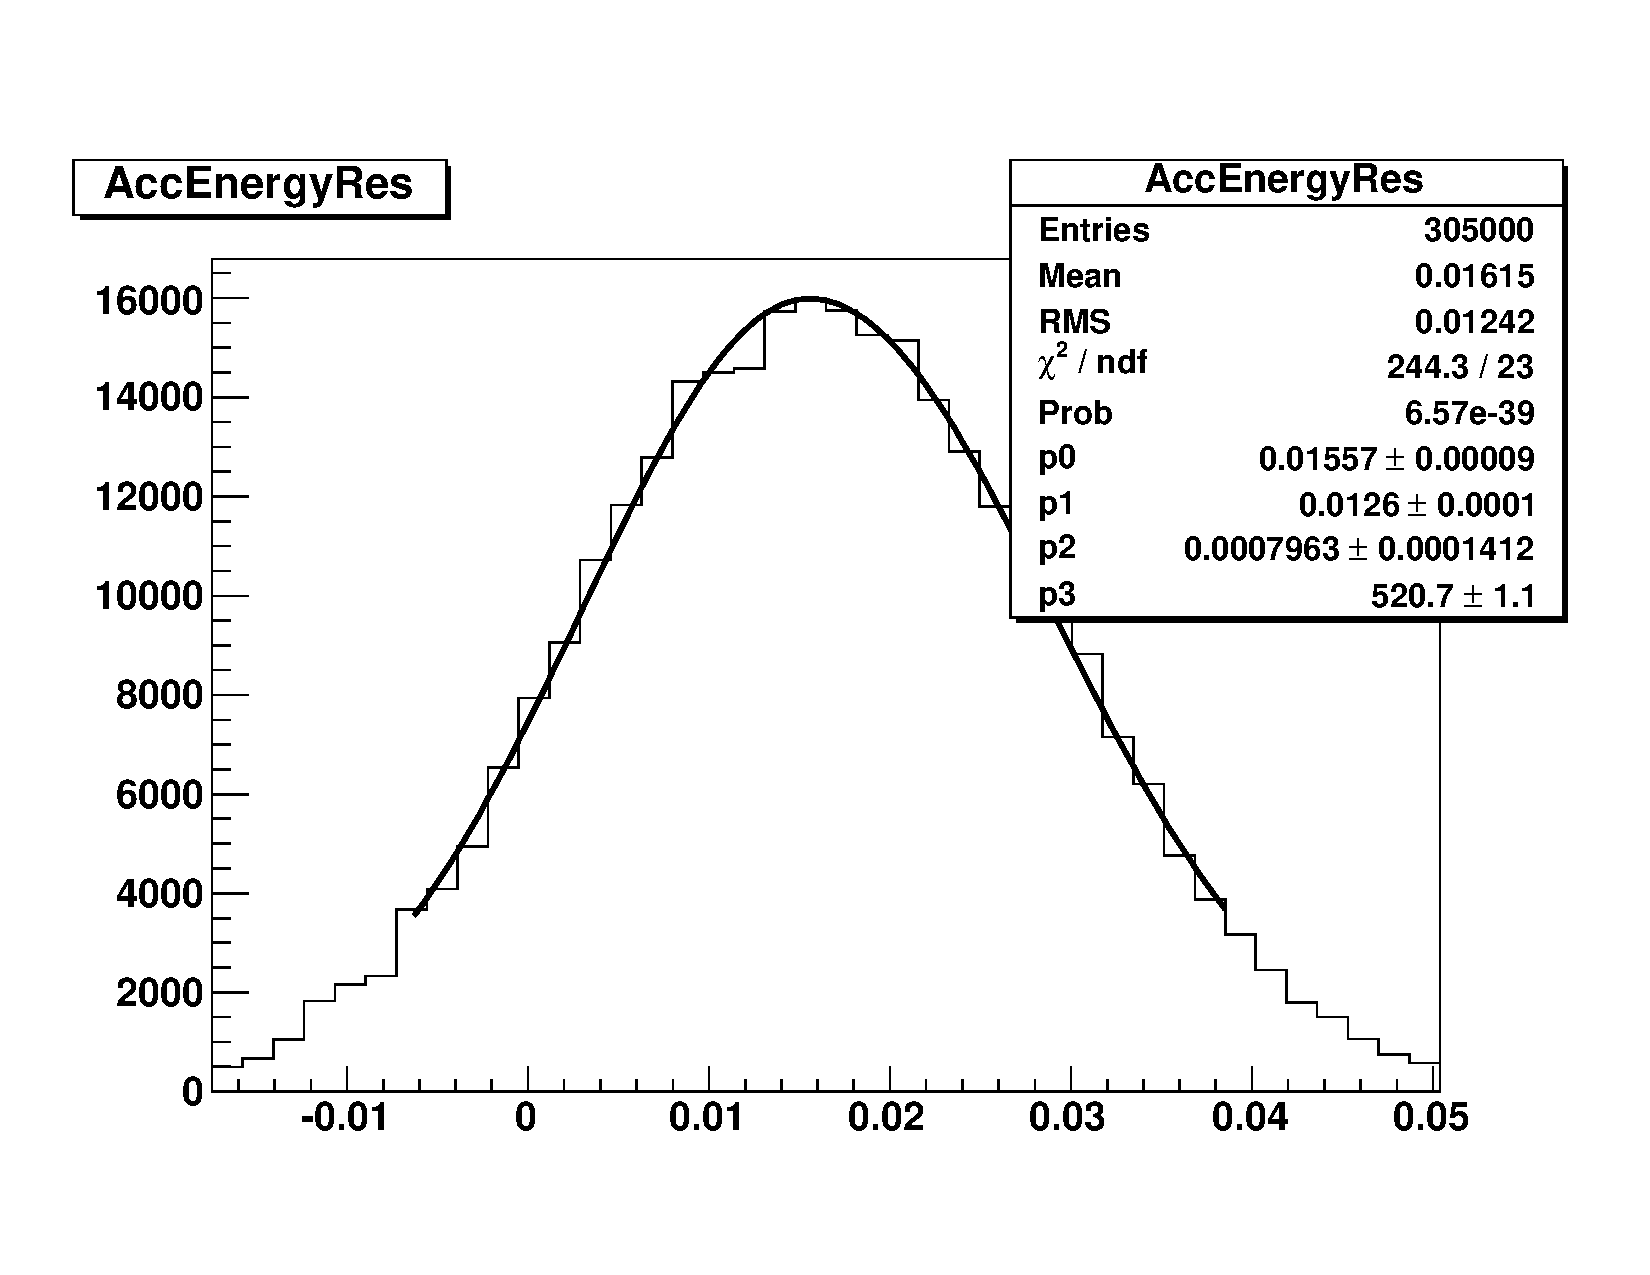
\includegraphics[width=0.8\textwidth]{Figures/MCMC/EnergyResPost}
\caption[Example posterior distribution]{An example posterior
distribution, with an asymmetric Gaussian fit.  This is the energy
resolution systematic from the final fit.
\label{FinalPostDist}}
\end{figure}


\section{Step Size Finding}
\label{rott:StepSizeFinding}
%Methodology - sweeps over orders of magnitude, typical plot, narrowing
%in, trade offs between decreasing $\tau$ and decreasing steps taken,
%target steps taken, autocorr measure of goodness.
In the MCMC process, at each step each parameter is varied by adding a
random draw from a Gaussian, with a different width for each
parameter.  These widths don't affect the theoretical behavior of the
chain, in the sense that any choice of widths will eventually produce
a random sampling of $p(\vec{\alpha}|\{\vec{x}\})$.  They do, however,
have a very large impact on the practical behavior of the MCMC.  

This can be illustrated by thinking about a case with one parameter,
for example one with the Likelihood versus parameter value shown in
\mbox{Figure \ref{LikelihoodExample}}.  Suppose we start our chain at
the point marked with an arrow.  The dimension marked $\sigma$ is a
reasonably good width for our Gaussian.  Since the Likelihood is steep
there, we are much more likely to take a step ``uphill'' and will
reach the maximum in a few steps.  More importantly, the region
containing most of the probability is only approximately ten
$\sigma$'s wide.  Once a parameter value near the maximum is reached,
the algorithm should have a good probability of stepping back
``downhill'' in one direction or the other, and thus exploring the
space around the maximum, as a step of size $\sigma$ will not change
the likelihood value too dramatically.  If the width were a tenth of
$\sigma$, however, we would have two problems: first, it would take
many steps to get to the maximum (this corresponds to a longer burn-in
period) and, once at the maximum, it would take a very large number of
steps to explore the majority of the probability.  If the width were
ten times $\sigma$, the opposite problem would occur: it would be very
likely that the step would take us away from the maximum completely,
and with a very low likelihood away from the maximum, that step would
be rejected by the algorithm.  We seek to balance between these
two cases.

\begin{figure}[tb]
\centering
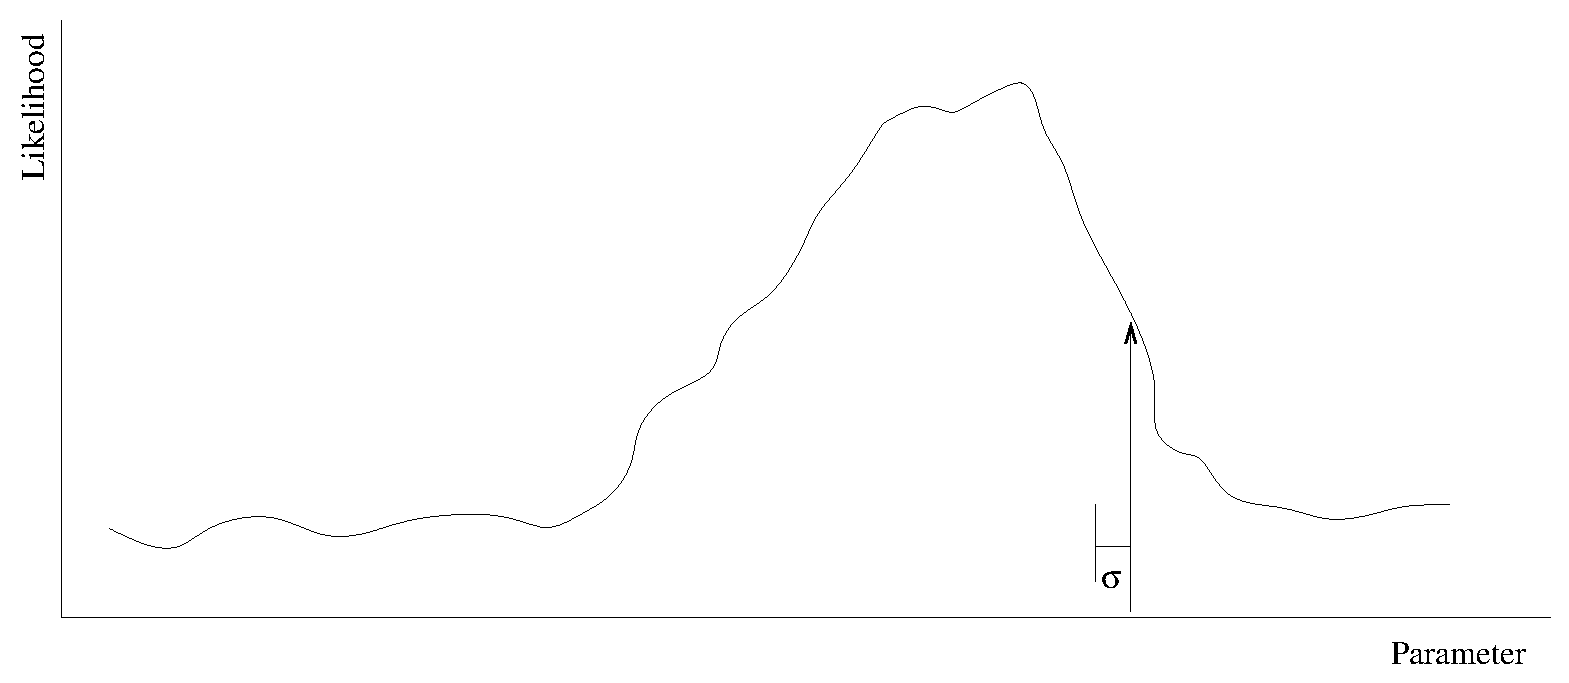
\includegraphics[width=0.8\textwidth]{Figures/MCMC/LikelihoodExample}
\caption[Example Likelihood v. parameter]{ An example of a possible
Likelihood versus parameter value graph, in the case of a system with
a single parameter.  See text for details.
\label{LikelihoodExample}}
\end{figure}

Looking at \mbox{Figure \ref{LikelihoodExample}}, we can immediately
see that the starting location of our chain plays a role.  Thankfully,
it can be proven that this role is transient, that is that regardless
of the starting point the chain will settle in to a proper sampling
$p(\vec{\alpha}|\{\vec{x}\})$ \cite{NealReport}.  We need to discard
this initial transient, called the burn-in period, as it is not part
of the sample we want.  The characteristic behavior of this burn-in
period is a rapidly changing log-likelihood, as the chain wanders
through low-probability regions where it is very probable for it to
take steps ``uphill''.  Once the chain reaches a high probability
region, the stable sampling behavior will set in; this is called a
stationary chain or stationarity.  This gives rise to graphs of
log-likelihood versus step such as \mbox{Figure
\ref{LikelihoodConvergence}}.  The end of the burn-in period is fairly
obvious on the graph, occuring around step 200, when the changes become
the size of the long-term fluctuations.  We customarily add 50\% or
100\% to the size of the burn-in period to be safe, as occasionally a
parameter will not have settled in to stationarity at that point, if
it has a very small impact on the likelihood.  Ideally, we should
check each parameter individually, but this is not practical when we
are dealing with hundreds of runs each containing dozens of
parameters.  Instead, we choose a few sample runs and check to make
sure the safety margin is sufficient.  We can, of course, force the
burn-in period to be shorter by moving the initial point closer to the
maximum likelihood point (as with any fitter).

\begin{figure}
\centering
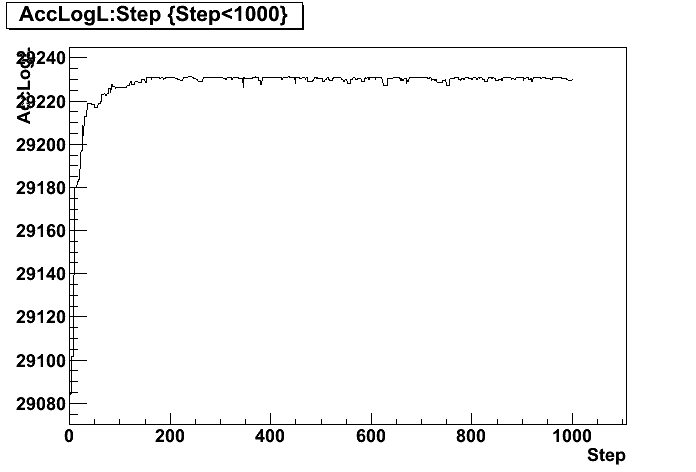
\includegraphics[width=0.8\textwidth]{Figures/MCMC/LogL}
\caption{Sample log likelihood v. step plot showing burn-in
\label{LikelihoodConvergence}}
\end{figure}

Before discussing how to optimize these step sizes, we need a goodness
measurement for our step sizes.  We seek to avoid two problems: too
large a step, which results in few steps taken, and too small a step,
which results in the space not being sampled properly.  The former is
simple to measure, we just measure how often the algorithm takes a
step.  Denote that ``\% steps''.  The rule of thumb is that it should
be roughly $23.4$\% for a system with multiple parameters
\cite{ref:DataAnalysisBook, DynamicStepPaper}, though the precision of
this number belies the range of acceptable values - any \% step
between 20\% and 30\% is quite good, and something between 15\% and
35\% is acceptable.  The latter problem is less obvious, but is well
measured by the autocorrelation.  This measures how many steps the
algorithm takes before values are no longer correlated with earlier
values, in colloquial terms how long before the chain ``forgets''
where it was before.  The smaller this is, the better we are sampling
the space, so it measures how independent our samples of
$p(\vec{\alpha}|\{\vec{x}\})$ are.  The autocorrelation is not an
indepedent measure from \% steps, as when very few steps are taken,
the chain ``remembers'' its location for a long time.  In fact,
\cite{ref:DataAnalysisBook, NealReport} point out that the
autocorrelation is the correct measure of what we desire in a chain,
while the \% step is just a useful rule of thumb.  We note, however,
that letting \% step get too small, even if it gives a better
autocorrelation, can unacceptably increase the burn-in period.
The autocorrelation is defined as
\begin{equation}
\rho(h) = \frac{\underset{t}{\sum} [(x_t - \bar{x}) (x_{t+h} - \bar{x})]}
  {\sqrt{\underset{t}{\sum} (x_t - \bar{x})^2 \cdot \underset{t}{\sum} 
    (x_{t+h} - \bar{x})^2}}
\end{equation}
where $x_i$ is an element in a sequence and $h$ is called the
``delay''.  $\rho(h)$ is equal to the traditional definition of
correlation between two sequences for the sequence $x_i$ and
$x_{i+h}$.  Note that this is only a useful measure once the burn-in
period has been removed, as we wish to measure the stationary sampling
behavior of the chain.  The autocorrelation should decay
exponentially, with a fluctuating background level due to the finite
number of points available.  A sample autocorrelation is shown in
\mbox{Figure \ref{GoodAutoCorr}}, which includes an exponential fit of
the form
\begin{equation*}
\rho(h) = A \exp(-\frac{h}{\tau})
\end{equation*}
The exponential's decay-time parameter $\tau$ gives us a single, real
number measure of the autocorrelation.  The smaller this $\tau$, the
faster the chain forgets its previous position, giving ``more
independent'' random draws from $p(\vec{\alpha}|\{\vec{x}\})$.

\begin{figure}
\centering
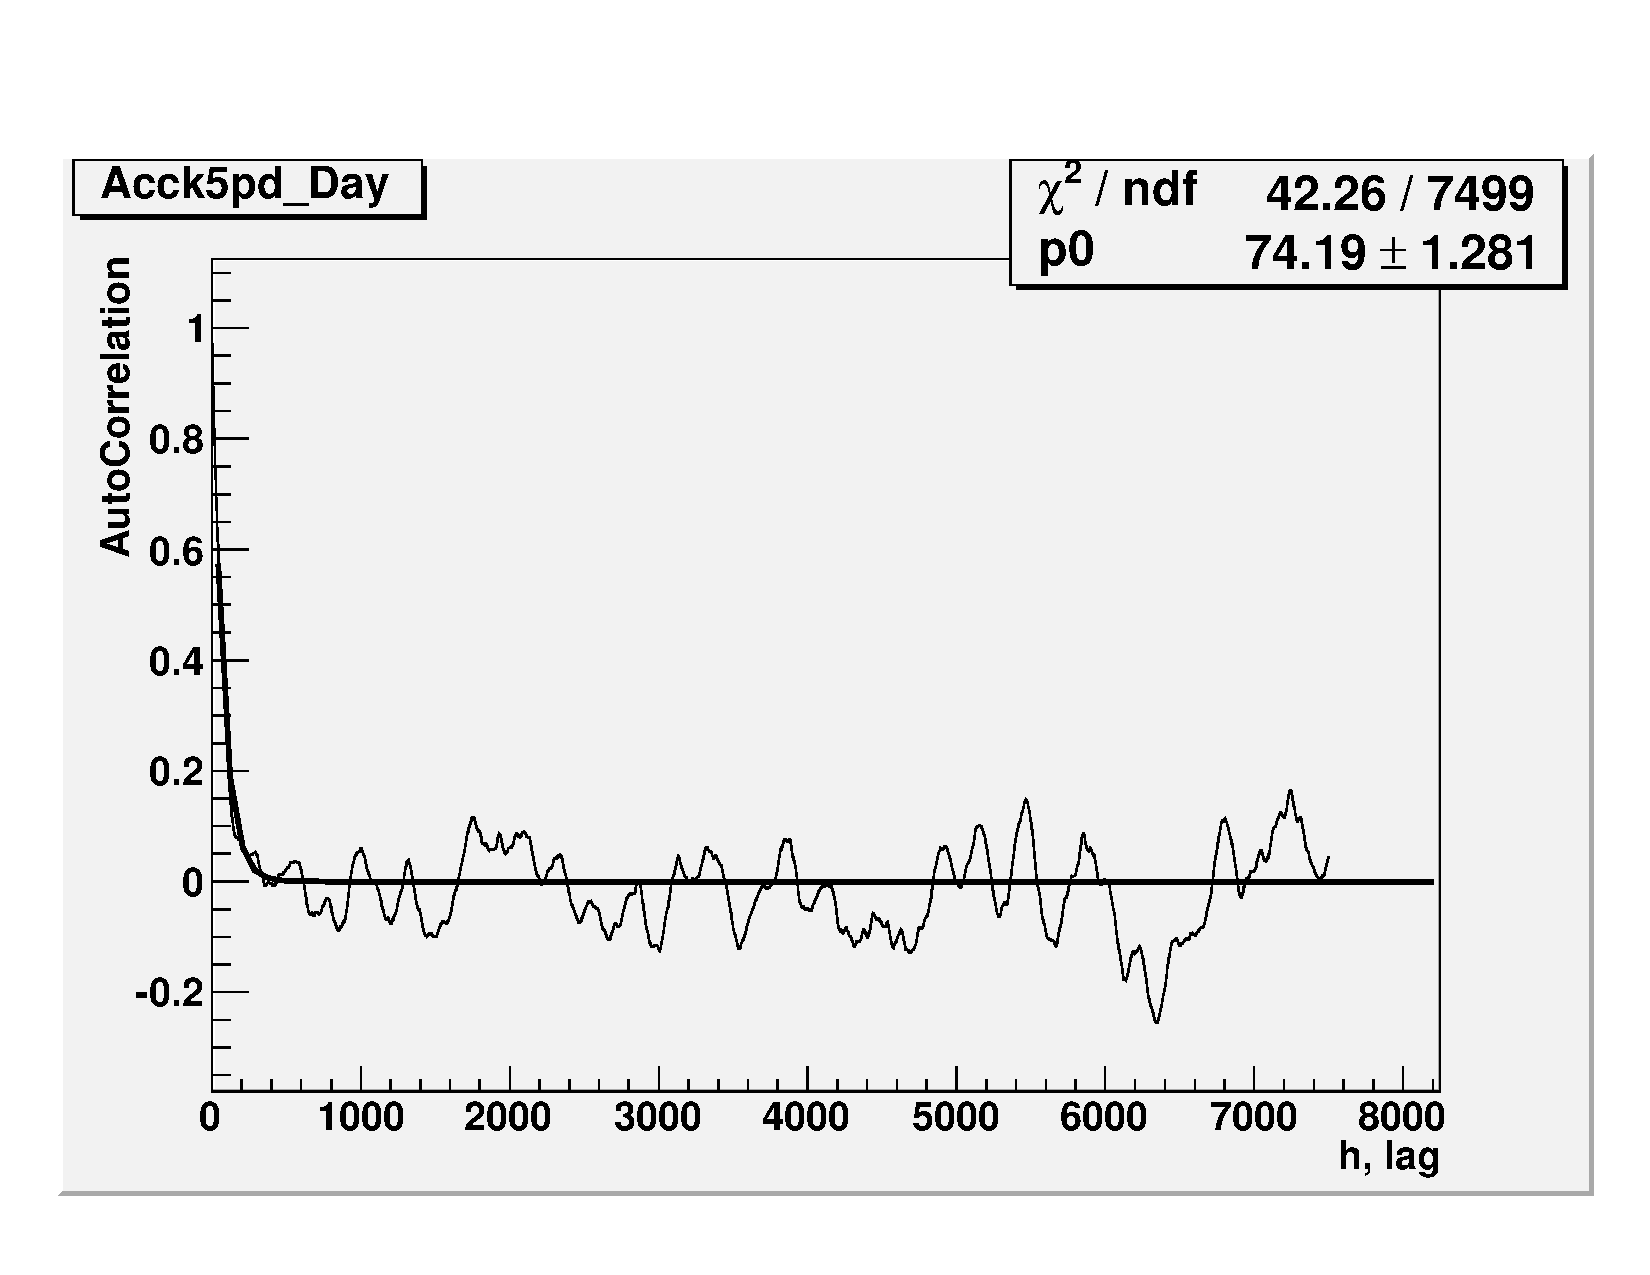
\includegraphics[width=0.8\textwidth]{Figures/MCMC/autoCorrGood}
\caption{Sample autocorrelation with exponential fit
\label{GoodAutoCorr}}
\end{figure}

We now seek to minimize $\tau$ for all parameters in our chain
simultaneously while keeping the \% step in an acceptable range.  A
way of automating this process is still an active area of research,
called Adaptive MCMC (see, for example, \cite{DynamicStepPaper}).
Having found no accepted method for finding the $\sigma_{\alpha_j}$'s,
through trial and error we settled on a methodology that, while a bit
slow and labor intensive, produces good results.  This method attempts
to make best use of our parallel computing resources by running many
chains with different step sizes in parallel at each step.  We will
refer to each instance of MCMC running in parallel as a ``run''.  Each
run has a fixed step size for each parameter.

We start by running a large sweep over possible step sizes.  Since we
are assuming to start with very little knowledge of the correct step
size, we will look over several orders of magnitude and sample
logarithmically, so that we get approximately the same number of
samples in each decade.  First we select a range to sample over for
each parameter.  In the case of a parameter with an external
constraint, this is straightfoward - the step size will be less than
the width of the constraint, but could be much smaller if the data
more sharply constrains it.  We will denote the constraint width as
$\delta$.  If we know nothing else about the system, we take a range
$[10^{-4}\delta,\delta]$.  We restrict this range if we have more
information, such as a similar system of parameters to compare
against.  In the case of a parameter with no constraint, we need to
guess.  If we have an idea of the ranges of values that we expect the
parameter to take, we use these in place of $\delta$, possibly
extending the range to $[10^{-6}\delta,10\,\delta]$.  Otherwise, we
simply run as broad of a sweep as we can, starting with a range of
$[10^{-8},10^{2}]$ when we run 100 runs in parallel (to keep about 10
runs per decade).  We may find we are still outside the range we want,
in which case we repeat with a different range.  We then randomly
sample within this range for each parameter, to generate a number of
runs with different step sizes.  We randomly choose instead of picking
a progression as the large number of parameters (over 50 in the main
analysis) would require a unacceptably large number of runs.  We then
run these in parallel, compute the autocorrelation for each parameter
and \% step for each run, and generate a plot of $\tau$ versus step
size and \% step versus step size for each parameter.  The burn-in
period can be a problem here, as it will vary for various step sizes.
We attempt to control for this by starting the chains as close to the
maximum as we can.  Since we do this step size finding process on
simulated data to avoid bias and blindness problems, we know the
actual maximum and can start arbitrarily close to it.  In addition,
those runs with too small a step size to find the maximum will return
very bad autocorrelations, which we need to keep in mind when looking
at results.

A sample $\tau$ plot is shown in \mbox{Figure \ref{SampleTau}}.  The
key characteristics to note are that $\tau$ tends to decrease as the
step size increases.  \mbox{Figure \ref{SampleFraction}} shows a
sample \% step versus step size plot.  Here we see that as step size
increases, \% step decreases.  This is the fundamental trade-off in
the step size finding process: increasing the step size of a parameter
decreases that parameter's autocorrelation, but decreases the \% step,
which increases the autocorrelation of all parameters.  We have found
that the ``corner'' in the $\tau$ graph, where $\tau$ stops decreasing
as quickly (about 0.4 in \mbox{Figure \ref{SampleTau}}, though we note
that the $\tau$ v. step size behavior is actually power-law like) is
approximately the best value.  We then find this corner for each
parameter and record it; we will denote this value $\varsigma$.  If
the corner is not present, we have not looked over a sufficiently
large range of step sizes so we repeat this step with altered ranges.

\begin{figure}
\centering
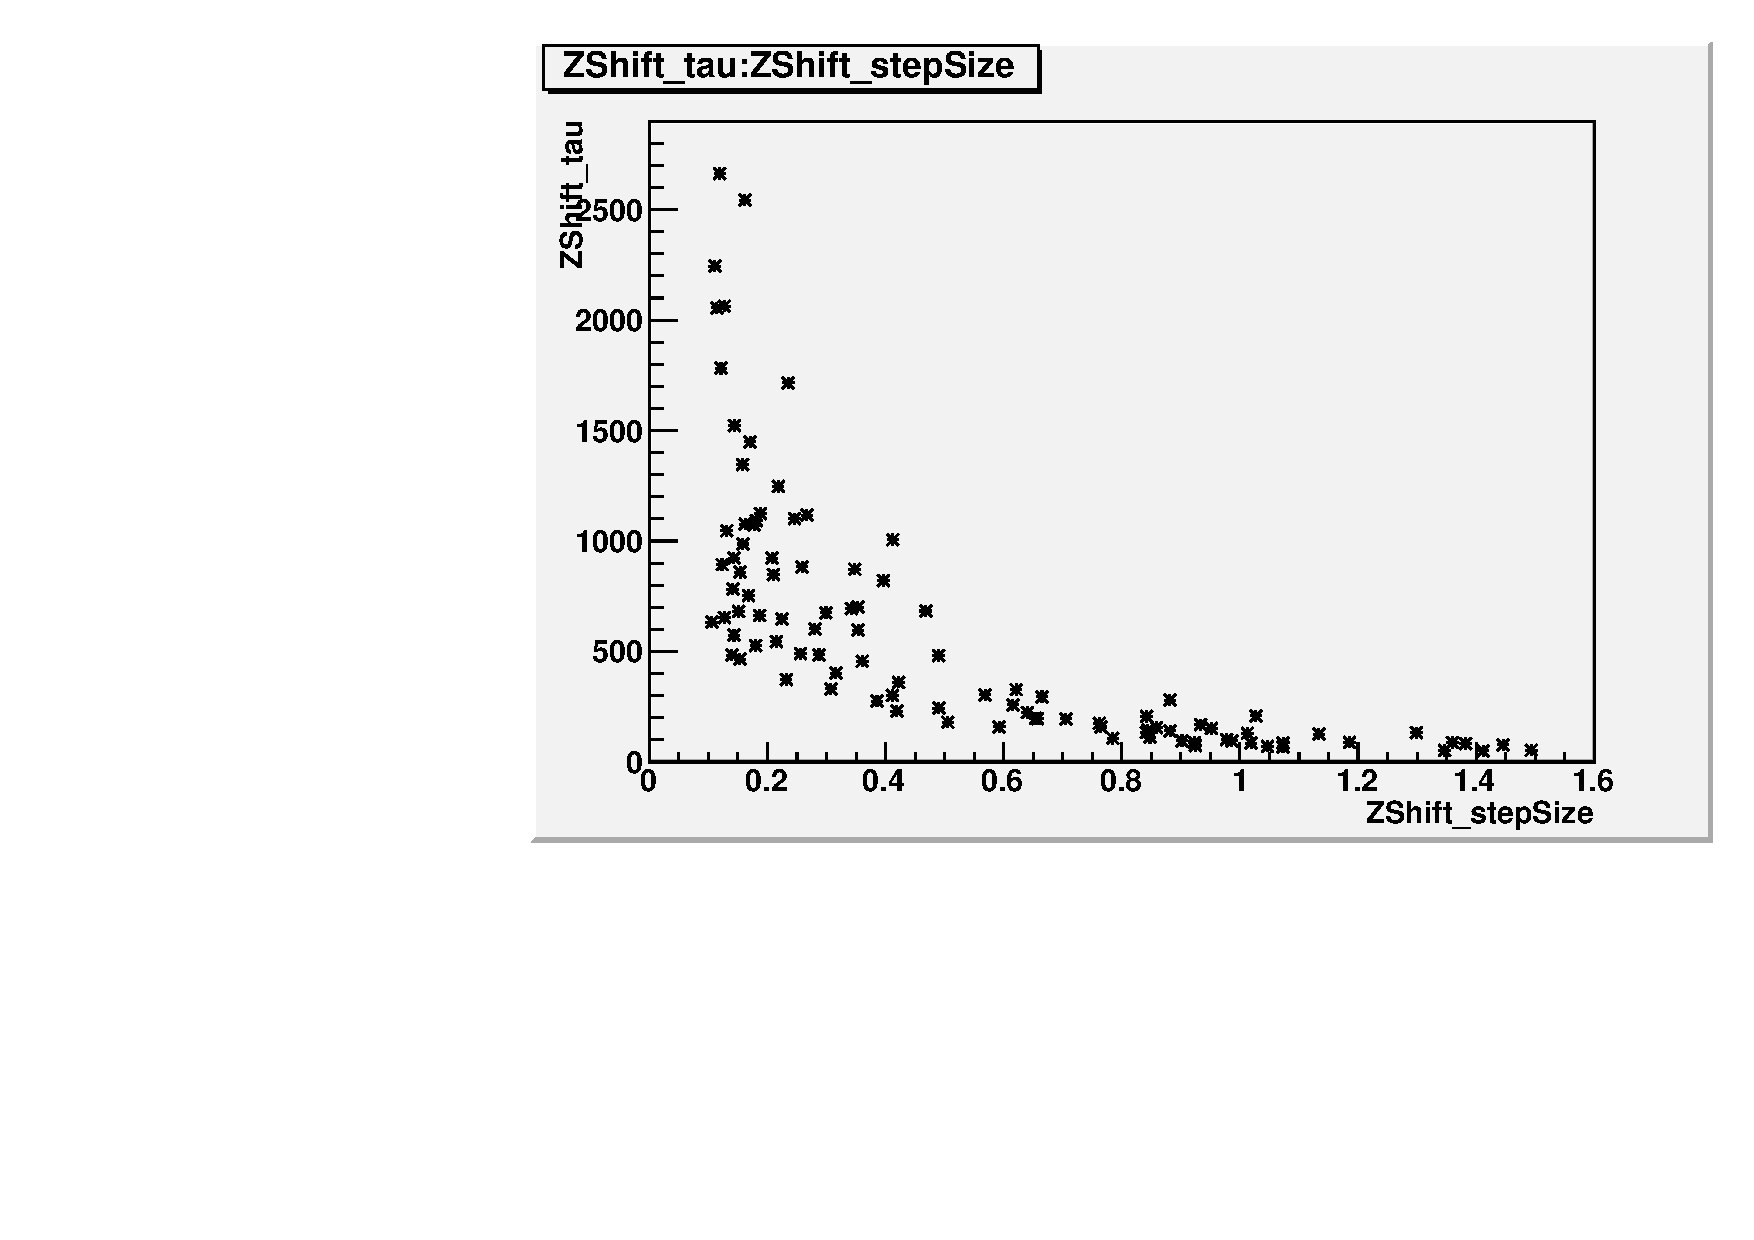
\includegraphics[width=0.8\textwidth]{Figures/MCMC/stepSizeLargeRangeTau}
\caption{Sample autocorrelation $\tau$ v. step size
\label{SampleTau}}
\end{figure}

\begin{figure}
\centering
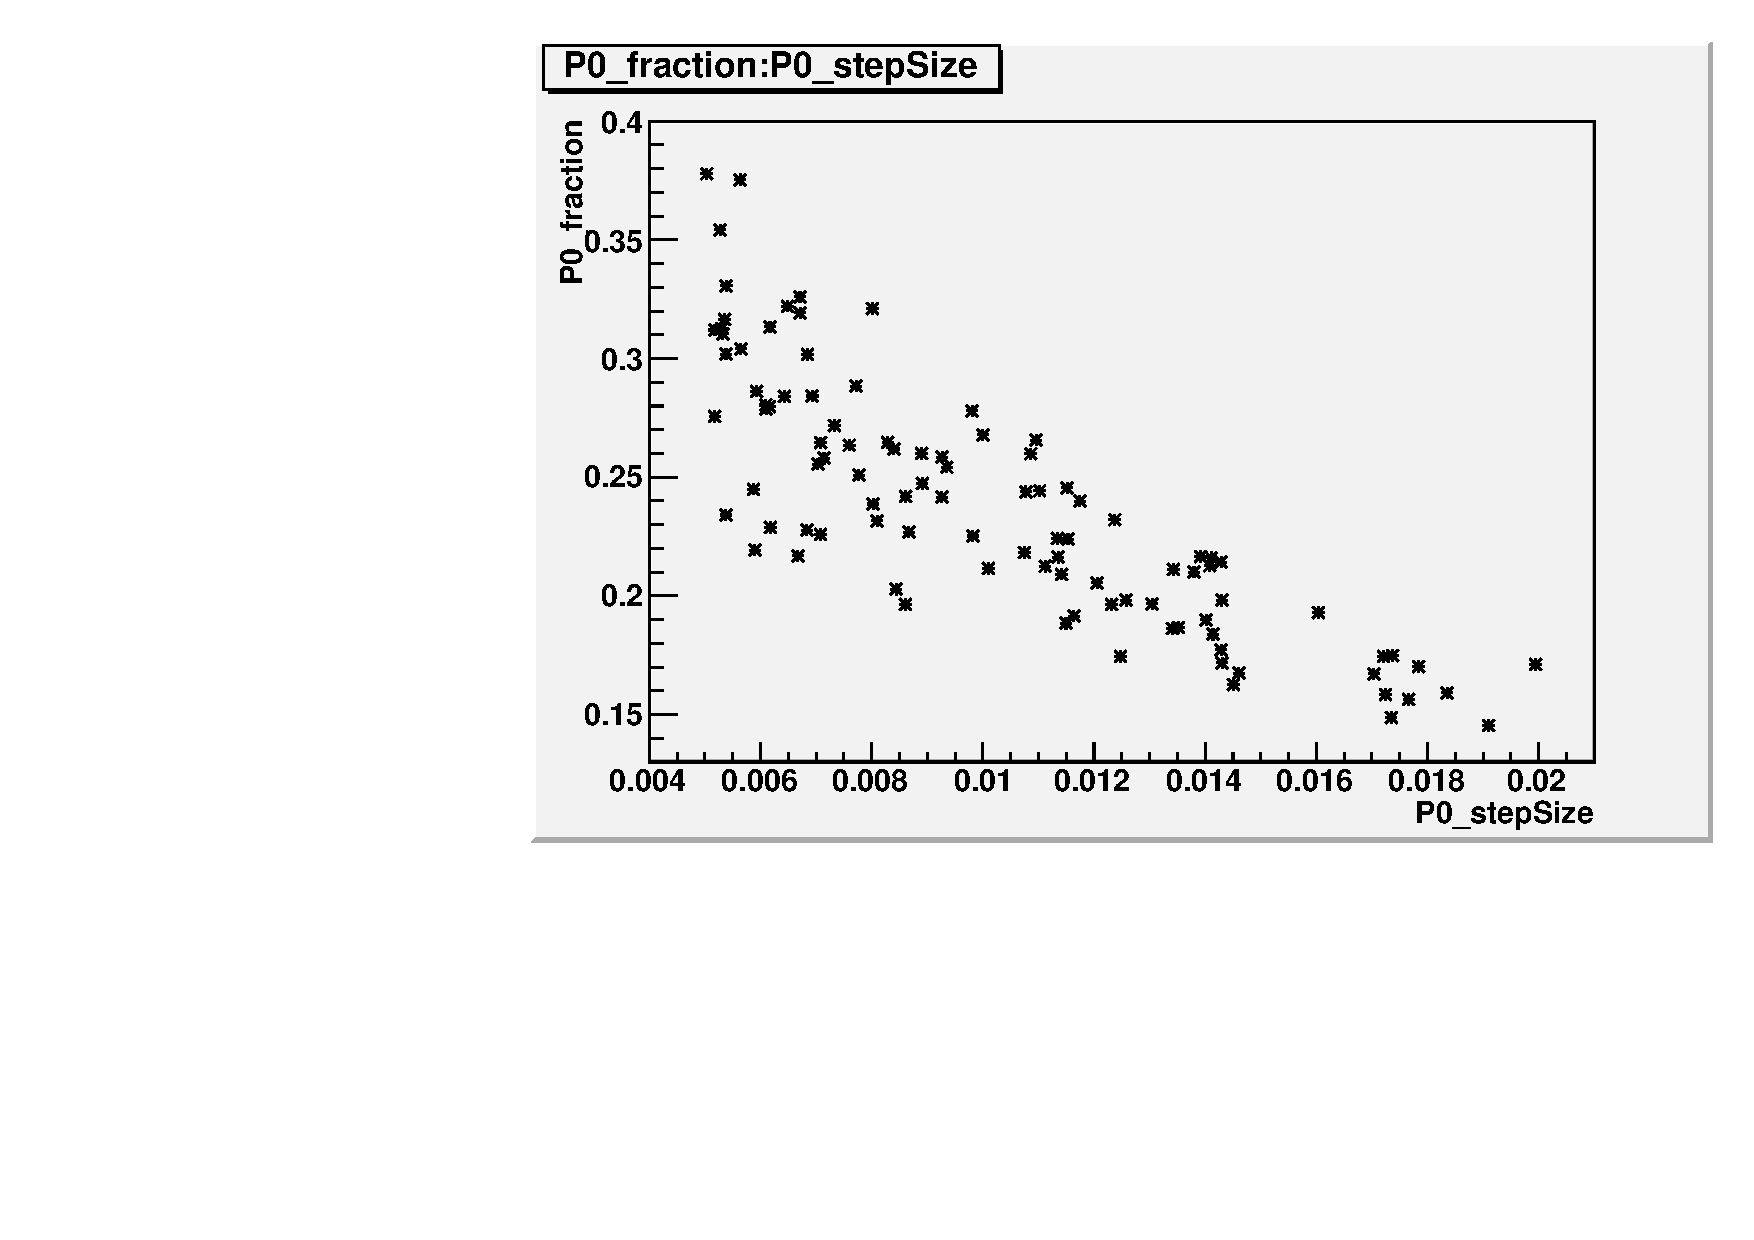
\includegraphics[width=0.8\textwidth]{Figures/MCMC/P0FractionVStep}
\caption{Sample \% step v. step size
\label{SampleFraction}}
\end{figure}

With the $\varsigma$'s in hand, we know approximately the correct
values.  Unfortunately, the $\tau$'s are correlated, both through the
\% step change and through the MCMC process itself.  Thus we must
search again, though on a more restricted range.  We again create runs
with logarithmically randomly selected step sizes for each parameter,
this time from the range $\frac{1}{3}\varsigma,3\varsigma $ (this is,
of course, arbitrary).  We again run these in parallel and compute the
autocorrelations.  Instead of graphing the results, we search though
them for those with desirable characteristics.  We search for two
types of runs: those with the smallest $\tau$'s (in particular ones
with all $\tau$'s less than a particular value, which we lower until
only a few runs qualify) and those with the most uniform $\tau$
values.  Ideally, we'll find a run with all $\tau$'s similar and
small, in the case of the final experimental run this was a $\tau$ of
approximately 200.  If we do, and this has a reasonable \% step, we
have found our step sizes and we stop.  If not, we look at the best
runs and see what needs to change.

If the runs are close to what we need, we adjust by hand and test.  In
the case of one or two parameters with too large $\tau$'s, we increase
the step sizes of those problem parameters and decrease the step sizes
of a few parameters with much lower $\tau$'s to compensate (unless the
\% step is too large, in which case we only increase).  If all of the
$\tau$'s are similar but too large, we look at the \% step.  If it is
too large, we increase all step sizes, if too small we reduce all step
sizes.  We must be careful here - if all of the $\tau$'s are much too
large, this can be the result of the autocorrelation not fitting well
to an exponential, for example \mbox{Figure \ref{BadAutoCorr}}.  This
usually arises from a run that hasn't actually passed through the
burn-in period, though it can also result from a run with a $\tau$ so
large that we simply did not run long enough to properly measure it.
We reject those runs, as they tell us nothing.  Either way, this gives
a new set of values, $\tilde{\varsigma}$.  We now again randomly
sample, this time of the linear range
$[\frac{1}{2}\tilde{\varsigma},\frac{3}{2}\tilde{\varsigma}]$, but
include an additional run with all parameter step sizes at
$\tilde{\varsigma}$.  We then repeat the search described in this
paragraph, adjusting as necessary and iterating.  This usually only
takes one or two iterations, but occasionally can become problematic.

\begin{figure}
\centering
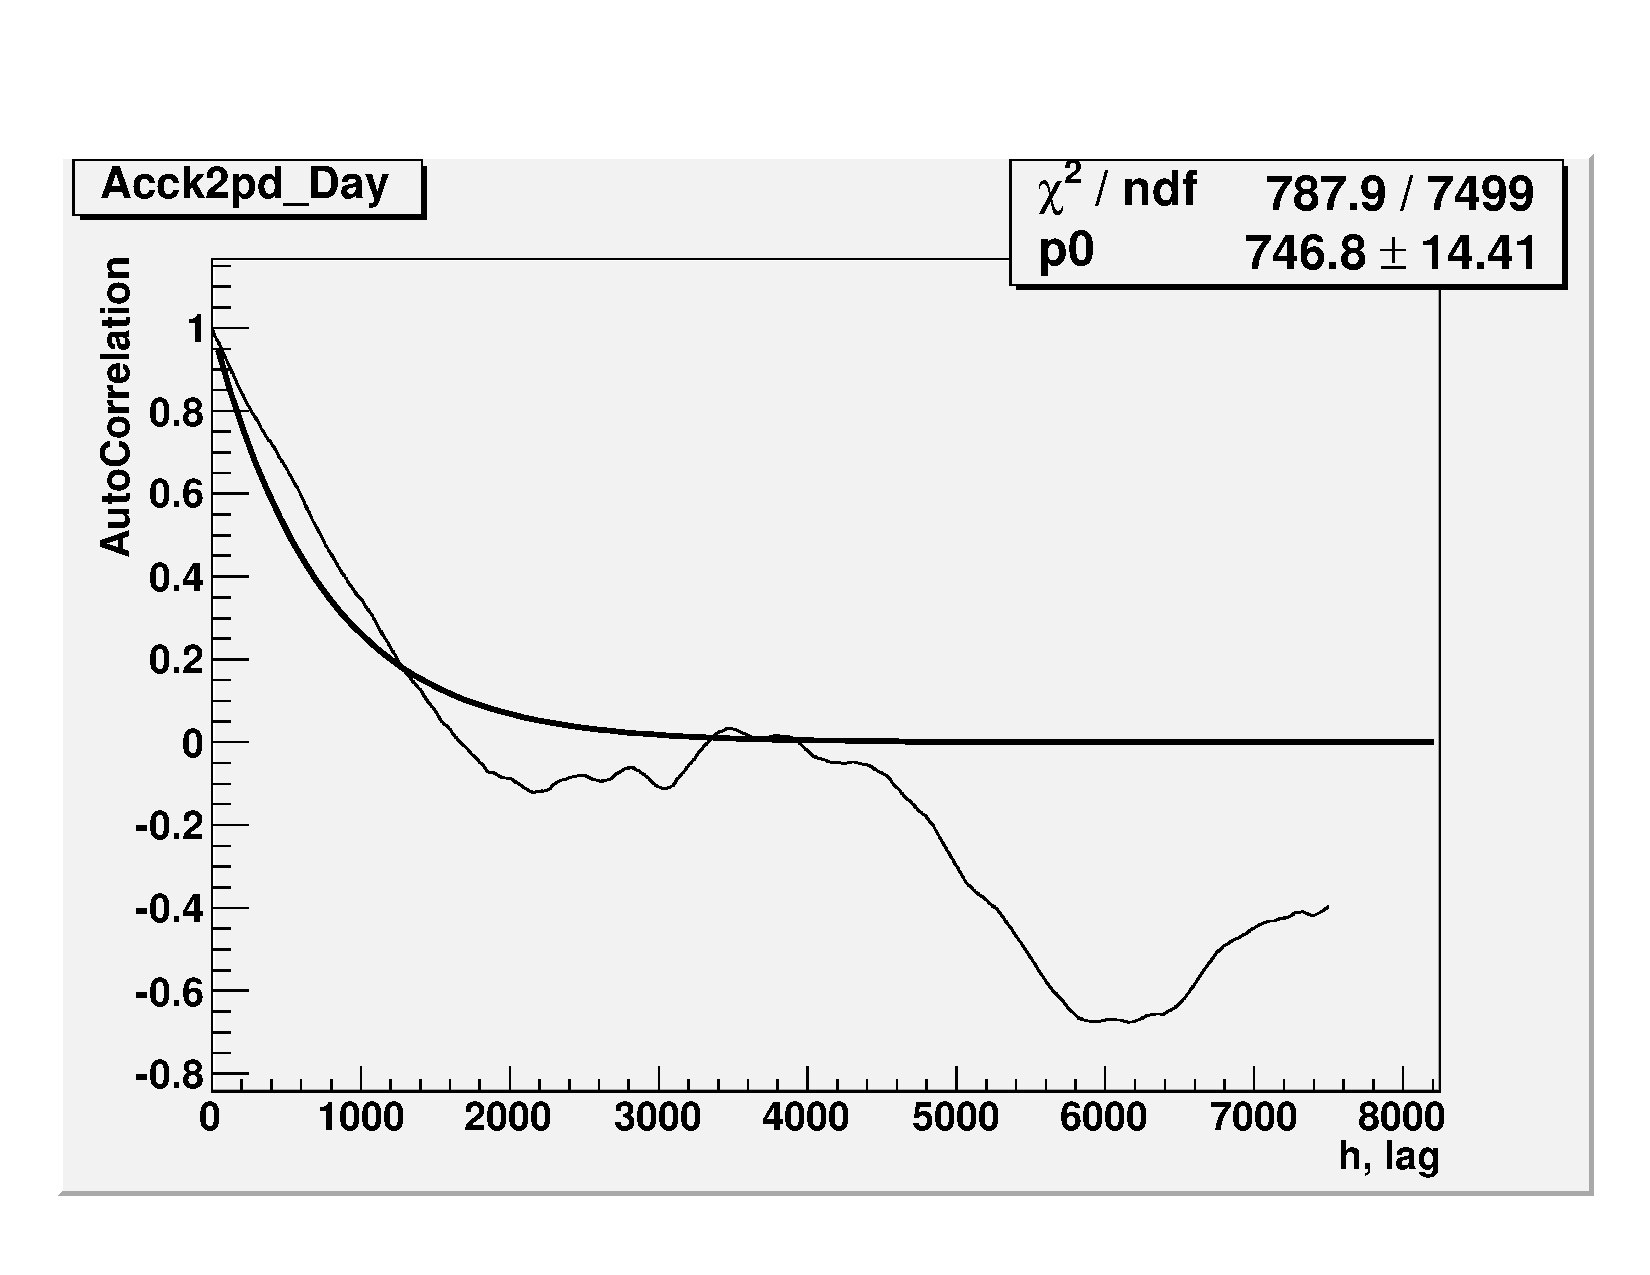
\includegraphics[width=0.8\textwidth]{Figures/MCMC/autoCorrBad}
\caption{Sample autocorrelation plot where exponential fit failed
\label{BadAutoCorr}}
\end{figure}

In an attempt to automate and streamline this process, we implemented
the Adaptive MCMC described in \cite{DynamicStepPaper}.  This is a
variant on the Metropolis algorithm which adjusts the step sizes
at each step, in an ever decreasing way.  This adjusts the MCMC
algorithm to
\begin{equation*}
\begin{split}
& \vec{\alpha}_{i+1}^{prop} = \vec{\alpha}_i + 
\vec{g}(\vec{\sigma}_{\vec{\alpha},i})\\
& p(\mathrm{step}) = \frac{EL(\vec{\alpha,i+1}^{prop})}
{EL(\vec{\alpha}_i)}\\
& \mathbf{if}\ \mathrm{rand}(0,1) < p(\mathrm{step})\\
& \ \ \mathbf{then}\ \vec{\alpha}_{i+1} = \vec{\alpha}_{i+1}^{prop}\\
& \ \ \mathbf{else}\ \vec{\alpha}_{i+1} = \vec{\alpha}_i\\
& \vec{\sigma}_{\vec{\alpha},i+1} = \vec{\sigma}_{\vec{\alpha},i} + 
\vec{\sigma}_{\vec{\alpha},0} (p(\mathrm{step})-0.234) i^{-\beta}
\end{split}
\end{equation*}
where $\beta$ is a real number controlling how quickly the adjustments
reduce in size, usually set somewhere between $0.5$ and $1$.  This is
a very simple change: we now have a variable step size, which we
adjust at every step, decreasing if the probability to take a step was
smaller than $23.4$\% and increasing if it was larger.  This serves to
force the algorithm to take \% step $=23.4$\%.  This algorithm, as
presented in the paper, has an unacceptable drawback: it changes all
the step sizes together.  This means that their relative proportions
never change.  This was the case for the example in the paper, but is
not the case for us.  We do not know beforehand what the ratios should
be, since some parameters affect the likelihood more than others.  To
correct this, we adjust this algorithm to only alter one parameter at
a time.  The algorithm behaves identically, save that the last line
now reads
\begin{equation*}
(\vec{\sigma}_{\vec{\alpha},i+1})_j =
(\vec{\sigma}_{\vec{\alpha},i})_j + (\vec{\sigma}_{\vec{\alpha},0})_j
(p(\mathrm{step})-0.234) i^{-\beta}
\end{equation*}
and j is incremented at each step, modulo the number of parameters, so
it walks through the parameter list from top to bottom repeatedly.

When we initially did this, we found that the first parameter was
being altered too much.  The size of the changes in
$\vec{\sigma}_{\vec{\alpha},i}$ is falling like $i^{-\beta}$, where we
used $\beta = 0.66$, which is $1$ for the first step, and
approximately $0.08$ by the end of the first pass through our roughly
$50$ parameter long list.  To correct for this, we instead keep the
size fixed for the first pass through the list: we have the first $m$
steps (where $m$ is the number of parameters) replace $i^{-\beta}$
with $m^{-\beta}$.

This altered algorithm does amazingly well at causing the chain to
settle in to a set of step sizes where \% step is $23.4$\%.
Unfortunately, there are many such sets of step sizes - this is a
single (albeit complicated) constraint in a high-dimensional space of
possible step sizes.  This adaptive algorithm did not produce useful
results, as it always found a region where some of the
autocorrelations were very small and some were very large.  We wound
up discarding it after many trials and reverting to the original
Metropolis algorithm with the step size finding procedure outlined
above.
%It might be possible, however, to
%make use of it in mapping out the high-dimensional sheet where \% step
%is some fixed percent, if that were desired.

\section{Benefits and drawbacks}
The most obvious strengths to this method are computational.  In
particular, it is an ``embarrasingly parallel'' algorithm - to run it
across multiple computers, we run an instance of the algorithm on each
machine.  They do not need to communicate.  We then simply take each
machine's output for $\{\vec{\alpha}\}$ (which will be different, as
this is an inherently random process) and concatenate them in to a
larger set.  This is in stark contrast to a deterministic Minuit-style
minimizer, which is extremely difficult to parallelize.  The only
catch to this is the burn-in period.  Each computer will individually
go through this process, so the first few events of each computer's
output chain must be removed before concatenation.  Even with that
being true, this easily allows much longer chains to be run.  For
instance, in this analysis we had access to a cluster of approximately
1500 nodes, called Tier2, of which we could reasonably expect to use
100 or so at a given time.  In the final analysis, we could run
approximately $7000$ algorithm steps in a 24 hour period.  With a
burn-in period of $2000$ steps, we were able to use a chain of
$305000$ events in a 24-hour run (not all 100 jobs ran due to computer
cluster problems), more than sufficient for good results.

In addition, the MCMC algorithm deals reasonably well with large
numbers of parameters.  The additional cost of an additional parameter
is very small, one random draw from a Gaussian per step.  The real
additional costs come from two places: adding an additional parameter
usually implies adding complexity to $p(\vec{x}|\vec{\alpha})$, which
can be expensive, and more parameters generally require a longer
burn-in period and chain length.  The longer burn-in period is from
adding a dimension to our parameter space, which slows the random walk
process.  The chain length increases because of the step size problem:
as more parameters are added, the probability of taking a step goes
down (assuming the additional parameters have a reasonably strong
influence on the $\mathrm{ELL}$), requiring smaller step sizes.

Another, less obvious benefit is that the MCMC deals well with systems
where the likelihood is very complicated.  If the likelihood is not
smooth near the maximum, as is the case for our SigEx, a typical
Minuit-type minimizer can easily get caught in a local maximum.  In
addition, since these fitters assume Gaussian-like behavior near the
minimum (corresponding to our maximum), they can get incorrect
uncertainties.  The MCMC, however, simply maps out the likelihood
space and is immune to these problems.  They will, instead, show up as
non-smoothness is $p(\vec{\alpha}|\{\vec{x}\})$, which is appropriate.
How to interpret this is a separate issue.  We found all of our
parameters to have posterior distributions sufficiently close to a
two-sided Gaussian near the maximum that we were comfortable fitting
that function to them and report a value
$\alpha_j\,^{+\sigma_+}_{-\sigma_-}$ for each.

From a statistical standpoint, a major benefit is that we get a random
sample of $p(\vec{\alpha}|\{\vec{x}\})$.  We can now compute any
quantity we like, such as the correlation between any pair of
variables, by simply computing that quantity on those two elements of
$\{\vec{\alpha}\}$.  In addition, when we histogram a single parameter's
value, we integrate across all other parameters.  This is in a rather
literal sense: when we do this, we get
\begin{equation}
p(\alpha_j|\{\vec{x}\}) = \idotsint p(\vec{\alpha}|\{\vec{x}\}) 
\mathrm{d}\alpha_1 \ldots \mathrm{d}\alpha_{j-1} \mathrm{d}\alpha_{j+1}
\ldots \mathrm{d} \alpha_m
\end{equation}
This is the correct way to treat nuissance parameters such as
systematics, as it correctly folds their contributions to the
likelihood in to the width of the distribution of the parameter,
including any correlations.  This then avoids complications associated
with correlated parameters, though if we want to give the point of
maximum likelihood rather than the most probable value for each
parameter, we need to fit a multi-dimensional function to the joint
distributions of those parameters we are concerned about.

The MCMC is not without drawbacks.  The most glaring is the issue of
finding step sizes.  This adds greatly to the complexity of running an
MCMC, though we hope that researchers will one day perfect an adaptive
MCMC that does not have this problem.  Another problem related to its
complexity is that, as a random process, it tends to be slower than a
deterministic fitter on simpler systems.  In addition, it is not
always clear when the burn-in period has passed, as the algorithm does
occasionally fall in to local minima.  It will wander out of them
eventually, but that can be much longer than is reasonable to wait.
This is unusual, thankfully, and can be tested by either starting many
parallel chains with different initial conditions or by running one
very long chain.  The last drawback we will mention is that since this
algorithm is less well understood than some other fitters,
interpreting the results is more difficult.  It is impractical to
report the full $p(\vec{\alpha}|\{\vec{x}\})$, except possibly for a
few parameters.  In addition, the expectation is that a single number
plus an uncertainty will be reported.  This is fine when
$p(\alpha_j|\{\vec{x}\})$ is well approximated by a Gaussian or
two-sided Gaussian near the maximum, but that is not always the case.

